% vim: ts=4 sts=4 sw=4 tw=80
% FIXME
% 这个附录翻译得很不好, 有很多问题.
\chapter{Vim 配置管理}
\label{chap:vim_configuration_alternatives}
\marginpar{215}

第 \ref{chap:personalizing_vim} 章介绍了 Vim 的主要配置文件, 随着
阅读的深入, 我们不断地往 \texttt{vimrc} 中添加新的配置信息, 最终, 配置文件
可能会变得非常混乱, 难以管理.

本章将介绍一些组织 \texttt{vimrc} 的方法, 从小技巧一直到整个
配置系统.

最后, 将会介绍如何在多个不同的计算机中使用同一个 \texttt{vimrc} 文件,
方法是在网络中保存一份副本.

\section{保持 vimrc 整洁的技巧}
\label{sec:tips_for_keeping_your_vimrc_file_clean}

\texttt{vimrc} 是用户设置 Vim 的核心文件, 如果没有它, 就只能使用系统中原有
的设置, 因此用户要时刻保持 \texttt{vimrc} 的整洁, 并及时更新, 只有这样, 用
户才能时刻知道文件中包含了哪些内容. 有时候, 用户可能没办法在文件中找到自己
想要的内容, 笔者就曾经遇到过这种情况, 当时我的 \texttt{vimrc} 超过了 2000 行,
到那时才意识到整洁的必要性. 保持 \texttt{vimrc} 整洁并组织良好的技巧有:
\marginpar{216}
\begin{enumerate}
	\item 保持 Vim 处于非兼容模式

	这个技巧可能并不会让 \texttt{vimrc} 更整洁, 至少不能马上看出来, 然而
	它却非常重要. 让 Vim 处于非兼容模式下就可以打开许多特性, 而这些特性
	会被很多技巧和脚本使用到. 所以, 最好在 \texttt{vimrc} 的第一行总是写上
	\texttt{set nocompatible}.
	
	\item 使用注释

	有时候, 用户会在 Vim 中改变一些设置, 然后再把设置添加到 \texttt{vimrc},
	过一段时间后, 当用户想要清理 \texttt{vimrc} 时, 就会发现自己已经记不住
	某段脚本是干嘛用的, 以及当初为什么要添加它, 甚至连代码是从哪儿来的都已经记不清
	了. 为了防止这种情况发生, 那就给新加的东西写上注释. 笔者建议在注释中包含这
	些内容: 代码的作用 (描述), 从哪儿得到的 (来源), 代码的原作者. 有了注释的
	帮助, 用户就能够方便地查询到代码的来源, 以及决定是否需要删除它们. 注释
	用引号开始, 比如 \texttt{"This is a comment}.

	\item 数据分组

	脚本通常需要一些额外的设置, 或者是用户想要为脚本中的某些功能设置一些额外
	的按键绑定 (映射). 为了能更方便地看出设置的归属, 最好为数据分组. 分组的
	条件有很多种, 笔者推荐以下这些 (按照在文件中出现的顺序, 从上到下排列):
	\begin{itemize}
	  \item 通用的全局设置
	  \item 自己私有的按键映射
	  \item 特定于脚本的设置, 按脚本分组
	  \item 其他设置
	\end{itemize}

	\item 使用多个文件
	
	有时候, \texttt{vimrc} 可能会变得非常巨大, 无论怎么组织都显得非常混乱. 对
	于这种情况, 最好把它切分成多个文件. 为了切分 \texttt{vimrc}, 首先把需要分
	出的内容剪切到另一个文件中, 文件名最好能描述出文件的作用, 然后在
	\texttt{vimrc} 中原来的位置用 \texttt{source} 命令从新文件读取命令.
	比如, 把和按键映射相关的设置命令都移动到 \texttt{mappings.vim},
	然后在 \texttt{vimrc} 中添加 \texttt{source \$HOME/.vim/mappings.vim}.

\marginpar{217}
    \item 测试时使用其他文件

    从前, 当笔者想要测试某段新的 Vim 脚本代码或者宏时, 通常会把它们添加到
    \texttt{vimrc} 的末尾, 在测试结束后, 笔者往往会忘记把它们删除, 经过一段
    时间后, \texttt{vimrc} 就充满了我的测试代码. 为了避免重蹈覆辙, 读者
    应该把测试代码写在另一个文件中, 然后用 \texttt{source} 命令执行文件中的
    测试代码. 如果觉得不错, 就把代码移动到适当的地方, 否则, 只要把文件删掉即
    可.

	\item 为不同的操作系统使用不同的文件

	如果读者也像我一样, 在多个不同的系统中使用 Vim, 可能会发现有些配置不能
	适应全部的系统. 原因可能是因为有些设置是和操作系统相关的, 又或者是硬件
	配置不一样, 比如说有些系统的屏幕比较小, 而另一些则比较大. 如果出现这样
	的情况, 最好把系统相关的设置写在不同的文件中, 然后把通用的文件拷到所有
	的系统中, 再把系统相关的配置文件拷到各自的系统中.
\end{enumerate}

如果读者能够严格遵守这些技巧, 就很有希望把 \texttt{vimrc} 保持在一个非常整洁
的状态下, 这样的话, 无论想修改什么内容, 你都能快速地找到.

\section{vimrc 配置系统}
\label{sec:a_vimrc_setup_system}

使用 Vim 时, 为了永久地更改某项配置, 用户需要打开配置文件, 修改后再保存. 如果
只是在 Vim 中修改, 而没有写到配置文件中, 程序退出后, 所有的修改都会丢失.

假如有这样一个脚本, 它提供了一个设置菜单, 用户在其中所做的修改在程序退出后
仍然有效, 那将会怎样? Jos van RisWick 就开发出了这样的脚本.

通过使用他的脚本, 并按照他的语法来创建 \texttt{vimrc}, 用户不仅可以使新的配置
持久化, 还可以根据向导的指引, 一步步地对配置加以修改.

脚本的实现方式是, 把配置项周围的注释作为设置向导中所显示的信息的占位符.
笔者发现这个脚本非常聪明, 而且和我们通常用的不太一样, 所以我们在这里简单地介绍
一下如何使用它.
\marginpar{218}

脚本的下载地址是 \url{http://www.vim.org/scripts/script.php?script_id=1894},
下载的压缩包中包含了下面这些文件:
\begin{itemize}
  \item \texttt{setup.vim}: 主要的脚本
  \item \texttt{array.vim}: 包含了处理字符串数组的函数
  \item \texttt{arrayg.vim}: 包含了处理全局字符串数组的函数
  \item \texttt{strfun.vim}: 包含了字符串处理函数
  \item \texttt{tableaf.vim}: 用来在配置系统中显示 tab leaf
\end{itemize}

安装脚本的方法是把压缩包解压到 \texttt{VIMHOME} 目录下, 解压后, 文件就自动
放到了 \texttt{plugin/} 子目录中.

现在, 用户就可以准备好修改 \texttt{vimrc}, 但是在修改之前最好做个备份.

在我们开始往 \texttt{vimrc} 添加设置之前, 先来看一下配置系统的使用语法. 前
面我们已经说过, 技巧就是配置项周围的注释. 这些注释包含了很特殊的语法, 这样
脚本才能知道这些注释是干嘛用的, 语法的基本规则是
\texttt{"|ID|tabname|text|command|extra|val1|val2|val3|}.

其中每一项的意义如下表所示:
\begin{center}
  \begin{tabular}{lp{30em}}
  \hline
  项名 & 意义 \\
  \hline
   \texttt{"}	& 开始一个注释 \\
   \texttt{ID}	& 一个标识符, 脚本可以用它来区分不同的配置组. 当脚本启动时,
     用户要告诉脚本应该处理哪个配置组 \\
   \texttt{tabname} & 应用配置的 tab 的名字 (在脚本中称为 leaf) \\
   \texttt{text} & 和配置相关的文本信息 \\
   \texttt{command} & 配置项所要执行的实际命令, 比如 \texttt{set textwidth=},
     注意, 不需要填上具体的值 \\
	\hline
  \end{tabular}
\end{center}
\marginpar{219}
\begin{center}
	\begin{tabular}{lp{30em}}
	\hline
	  \texttt{extra} & 比如说, 如果命令是一个映射, 则变量部分就是被映射的
	  按键, 这时候用户还需要设置映射到的命令, 命令就是填在 \texttt{extra} 字
	  段中, 如果不需要它, 就留空 \\

	  \texttt{val1}-\texttt{val3} & 命令参数的默认值, 在配置系统中可以按
	  Tab 键来遍历这三个值. \\
	\hline
	\end{tabular}
\end{center}

再在来看一个例子:
\begin{vimcode}
"|SETTINGS|Layout|Set the text width|set tw=|50|70|90|
set tw=60
"|SETTINGS|Layout|Show a ruler?|let &ruler=||0|1|
let &ruler=1
\end{vimcode}
这个例子展示了设置 Vim 的两种典型方法 --- 用 \texttt{set} 与 \texttt{let} 来
设置一个选项. 在变量名左边加上 \texttt{\&} 是在告诉 Vim 等号右边的表达式要在
设置之前求值, 如果求值结果的类型和选项不一致, 还会自动转换类型. 注释下面是真
正的设置命令.

如果只是想在 tab 中添加一个注释, 只需要把命令替换成 \verb'%', 比如:
\begin{vimcode}
"|SETTINGS|Layout|Here you will find layout settings|%|
\end{vimcode}
用户还可以利用它来插入空行, 这些空行将作为间距来使用, 方法是用空格替换掉文本.

接下来讨论如何设置脚本.

设置脚本的地方在 \texttt{setup.vim}, 在脚本中搜索 \texttt{HERE2}, 找到该单词
出现的第二个地方, 你将会看到:
\begin{vimcode}
" Import settings from these files HERE2:
let setup_files=Arr("settings.vim", "mappings.vim", "scripts.vim")
let setup_group="SETTINGS"
\end{vimcode}
\marginpar{220}

\texttt{setup\_files} 是一个数组, 数组中的每一个元素都是一个文件名, 文件包含
了设置信息. 在上面的例子中, 我们用到了 \texttt{settings.vim},
\texttt{mappings.vim}, \texttt{scripts.vim} 这三个文件.

第二条命令告诉脚本当前设置使用哪一个配置组. 在示例中我们用的是
\texttt{SETTINGS}, 因此如果某个设置的注释以 \texttt{|SETTINGS|} 开始, 那么这
个设置就会被用到.

在开始使用配置向导之前, 在 \texttt{setup.vim} 中还有一项需要修改.

由于设置分散在多个文件中, 我们需要让 Vim 意识到这点, 因此 \texttt{vimrc} 要
包含 (在 Vim 中称为 source) 这些文件, 除此之外, 为了让修改生效, 还要让 Vim
重新加载 \texttt{vimrc}, 为了处理这种情况, 我们也提供了一个特殊的设置.

在 \texttt{setup.vim} 中搜索 \texttt{HERE1}, 找到单词出现的第二个地方, 用户
将会看到:
\begin{vimcode}
autocmd bufleave _setup source ~/.vimrc
\end{vimcode}
当用户离开配置向导时就会执行 \verb'source ~/.vimrc'. 如果需要的话, 用户
还可以添加其他外部配置文件.

现在讨论如何启动 Vim 配置向导, 并在向导中导航. 为了启动配置向导, 先切换到普通
模式, 然后按下 \texttt{s}, 启动后, 光标位于第一个 tab 的第一个设置上. 在向导
中有很多快捷键可以使用:
\begin{center}
  \begin{tabular}{ll}
    \hline
	快捷键  & 描述 \\
    \hline
    \texttt{r} 或 \texttt{R}  & 进入替换模式 \\
	\texttt{s} & 保存后退出 \\
	\texttt{q} & 不保存退出 \\
	\texttt{<space>} & 遍历所有的 tab leaf \\
	\texttt{j} & 跳转到当前 tab leaf 的下一个设置 \\
	\texttt{k} & 跳转到当前 tab leaf 的前一个设置 \\
	\texttt{<tab>} & 显示被选中的设置的可选值 \\
	\texttt{<cr>} & 接收当前行的修改 \\
	\texttt{<esc>} & 重新绘制当前的 tab leaf (普通模式) \\
	\texttt{<esc>} & 丢弃修改 (插入或替换模式) \\
	\hline
  \end{tabular}
\end{center}
\marginpar{221}

使用配置向导的准备工作就是这些. 下面的截图展示了向导的使用效果:
\begin{center}
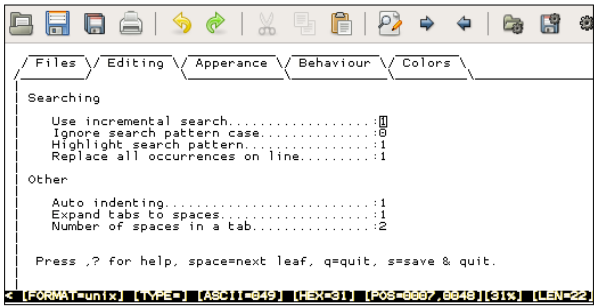
\includegraphics[scale=0.6]{./images/page221.png}
\end{center}

\section{在线存放 vimrc}
\label{sec:storing_vimrc_online}

假设用户要在多种不同的计算机中使用 Vim, 可能会因为每次都要重新设置 Vim, 或者
使用不同的设置而感到很恼火.

现在, 几乎每一台计算机都连接到了因特网上, 所以一个明显的解决办法是在线保存一
份 \texttt{vimrc}. 我们之前已经说过 Vim 可以编辑远程主机上的文件, 但是, 如果
要读取远程主机上的 \texttt{vimrc} 将会遇到一些问题. 通常情况下, 当 Vim 需要
读取网络上的文件时, 它会用到插件 \texttt{netrw}, 然而, 当 Vim 读取
\texttt{vimrc} 时, 这个插件还没有加载, 也就无法读取远程主机上的 \texttt{vimrc}.

解决办法是使用下面的函数:
\begin{vimcode}
function! GetNetVimrc(vimrc_url)
    source $VIMRUNTIME/plugin/netrwPlugin.vim
    Nread a:vimrc_url
    let tmpfile = tempname()
    save! tmpfile
    source tmpfile
    delete(tmpfile)
    enew
endfunction
\end{vimcode}
\marginpar{222}
读取 \texttt{vimrc} 的所有操作都在 \texttt{GetNetVimrc} 中完成. 函数的输入参数是
\texttt{vimrc} 的 URL 地址, 函数开始时先加载 \texttt{netrw} 插件, 加载后
Vim 就可以使用网络读写功能, 然后, 调用 \texttt{Nread} 从网络上读取
\texttt{vimrc} 到当前缓冲区, 再把文件的内容写到一个临时文件, 加载它, 最后再
把临时文件删掉, 并打开一个干净的缓冲区.

那么, 用户应该如何使用 \texttt{GetNetVimrc}?

首先把 \texttt{vimrc} 保存到网络上的某台主机, 如果用户想要在某个系统中使
用自己的在线 \texttt{vimrc}, 就把 \texttt{GetNetVimrc} 添加到系统本地的
\texttt{vimrc}.

调用函数的方式是:
\begin{vimcode}
:call GetNetVimrc("http://www.domain.com/myvimrc")
\end{vimcode}
还可以把上面这行代码添加到包含 \texttt{GetNetVimrc} 的 \texttt{vimrc} 文件中.

现在, 用户所有系统中的 Vim 都具有了相同的配置, 如果在线的 \texttt{vimrc} 有
了更新, 那么等下一次用户使用系统时, 这些更新也会反映在系统中.

记住, 用户还可以用 \texttt{Nread} 和 \texttt{Nwrite} 这两个函数来直接修改
在线 \texttt{vimrc}.

% end of appendix B
